\chapter{Templates}




\section{Boat}

\begin{figure}%
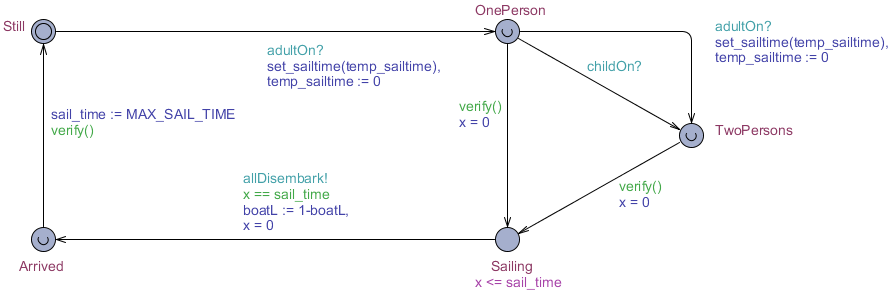
\includegraphics[width=\columnwidth]{pictures/boat.png}%
\caption{}%
\label{}%
\end{figure}
















\section{Person}
\begin{figure}%
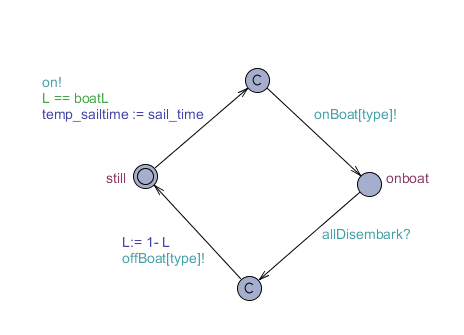
\includegraphics[width=\columnwidth]{pictures/person.png}%
\caption{The timed automata for a person}%
\label{fig:person}%
\end{figure}
The person model encapsulate a single person.
When instantiated it takes three arguments.
These arguments determines which type of person is being instantiated and how it should interact with the rest of the system.
The arguments that a person needs to be instantiated are: A channel, a person type, and a sail time.
The channel argument is used to signal that the given instance gets on the boat.
The person type indicates what kind of person is being instantiated, e.g. a boy.
The sail time is only applicable to the mom, dad, and police officer.
It is part of the 2nd task, which is to add temporal constraints and have each of the adults cross the river with different speeds.

The timed automata of a person seen in Figure \ref{fig:person} shows four circular connected locations.
The two locations OnBoat and OnLand indicate the current position of the person.
These names should be self-explanatory.
The locations ToBoat and ToLand are intermediate states.
These are needed because there is a handshake with the boat and a broadcast to the observer whenever a person embarks or disembarks.
When a person 















\section{Observer}
\begin{figure}%
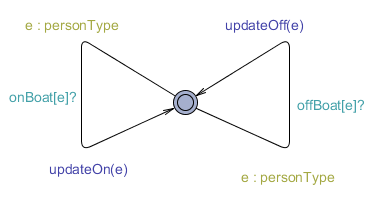
\includegraphics[width=\columnwidth]{pictures/observer.png}%
\caption{}%
\label{}%
\end{figure}




























\section{Observer}